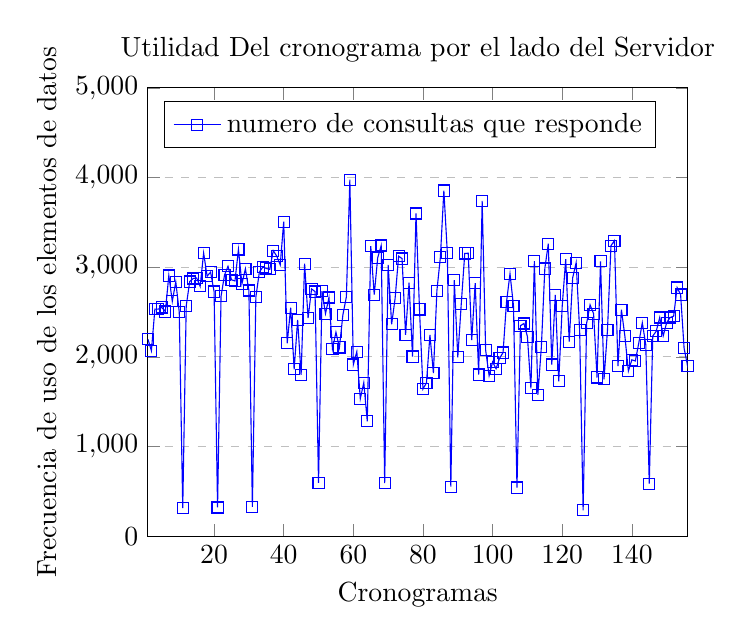
\begin{tikzpicture}
\begin{axis}[
    title={Utilidad Del cronograma por el lado del Servidor},
    xlabel={Cronogramas},
    ylabel={Frecuencia de uso de los elementos de datos},
    xmin=1, xmax=156,
    ymin=0, ymax=5000,
    xtick={},
    ytick={},
    legend pos=north west,
    ymajorgrids=true,
    grid style=dashed,
]

\addplot[
    color=blue,
    mark=square,
    ]
    coordinates {
%UTILIDAD total
(1,2197)
(2,2068)
(3,2533)
(4,2532)
(5,2551)
(6,2505)
(7,2907)
(8,2619)
(9,2837)
(10,2499)
(11,314)
(12,2568)
(13,2840)
(14,2874)
(15,2880)
(16,2786)
(17,3158)
(18,2900)
(19,2945)
(20,2728)
(21,320)
(22,2675)
(23,2913)
(24,3010)
(25,2860)
(26,2847)
(27,3198)
(28,2815)
(29,2982)
(30,2740)
(31,327)
(32,2666)
(33,2944)
(34,3002)
(35,2986)
(36,2976)
(37,3184)
(38,3124)
(39,3025)
(40,3508)
(41,2152)
(42,2549)
(43,1861)
(44,2412)
(45,1798)
(46,3040)
(47,2432)
(48,2757)
(49,2728)
(50,594)
(51,2732)
(52,2482)
(53,2662)
(54,2090)
(55,2275)
(56,2105)
(57,2469)
(58,2669)
(59,3976)
(60,1914)
(61,2058)
(62,1533)
(63,1712)
(64,1281)
(65,3234)
(66,2694)
(67,3106)
(68,3242)
(69,593)
(70,3026)
(71,2364)
(72,2653)
(73,3123)
(74,3096)
(75,2246)
(76,2827)
(77,2003)
(78,3599)
(79,2529)
(80,1642)
(81,1709)
(82,2245)
(83,1820)
(84,2738)
(85,3111)
(86,3855)
(87,3157)
(88,552)
(89,2855)
(90,1994)
(91,2592)
(92,3153)
(93,3156)
(94,2186)
(95,2823)
(96,1803)
(97,3740)
(98,2075)
(99,1790)
(100,1944)
(101,1868)
(102,1984)
(103,2048)
(104,2613)
(105,2928)
(106,2567)
(107,542)
(108,2348)
(109,2372)
(110,2226)
(111,1650)
(112,3067)
(113,1577)
(114,2107)
(115,2985)
(116,3262)
(117,1914)
(118,2691)
(119,1728)
(120,2569)
(121,3090)
(122,2170)
(123,2882)
(124,3051)
(125,2297)
(126,288)
(127,2374)
(128,2580)
(129,2482)
(130,1770)
(131,3065)
(132,1749)
(133,2302)
(134,3240)
(135,3296)
(136,1896)
(137,2525)
(138,2229)
(139,1842)
(140,1967)
(141,1954)
(142,2157)
(143,2380)
(144,2135)
(145,585)
(146,2232)
(147,2286)
(148,2439)
(149,2234)
(150,2382)
(151,2439)
(152,2454)
(153,2773)
(154,2695)
(155,2097)
(156,1900)
(157,2190)
(158,2275)
    };
    \legend{numero de consultas que responde}

\end{axis}
\end{tikzpicture}

